\chapter{Methods}\label{chap:methods}

% Describe the method/software/tool/algorithm you have developed here

In the preceding chapters, all the necessary background knowledge to understand the methods have been introduced. In this chapter, we will present an overview of the challenges, the methods, and the tools we have developed for this thesis. We will first describe the dataset we have used for this thesis. Then, we will describe the programs we have developed for this thesis. Finally, we will describe how we have packaged and deployed our programs with Nix.


% * collaboration between clément and I
% * timeline of the project
% * the architecture for computations, personal machine, remote server
% * packaging and deployment with Nix

\section{Dataset exploration}
The dataset that serves as the basis for this thesis has been introduced before (see \autoref{sec:background:kex:dataset}). At his heart, the dataset is a collection of heap dump RAW files for different use cases and versions of OpenSSH. Each heap dump file goes along a JSON annotation file that has been generated by the creators of the dataset to provide additional information about the heap dump, and especially encryption keys. In this section, we will describe the dataset exploration we have done to get a better understanding of the dataset. 

    \subsection{Estimating the dataset balancing for key prediction}
    First, let's quickly estimate what the dataset is composed about. This will later be used to estimate the balancing of data for our key prediction goal. Some quick linux commands can be used to get a general overview of the dataset.
    
    A first command can quickly give us an idea of the number of files in the dataset:
    \begin{lstlisting}[caption={Count all dataset files}, label=methods:code:count_all_dataset_files, language=bash]
        find /path/to/dataset -type f | wc -l
    \end{lstlisting}

    Another command can be used to get the total size of the dataset:
    \begin{lstlisting}[caption={Get the total size of the dataset}, label=methods:code:get_total_size_dataset, language=bash]
        du -sb /path/to/dataset
    \end{lstlisting}

    The first command indicates that the dataset contains $ 208749 $ files, which represents, according to second one, a total of $ 18203592048 $ bytes, or around 18 Gigabytes.

    We could just divide the number of files by the size of the dataset to get an average size of the files. However, this would not be accurate, as we are only interested in the size of the RAW files. Since JSON files are much smaller than RAW files, they would skew the average size of the files. Since we are only considering RAW files, we will use improved commands in order to determine the size of the RAW file only.

    The following command can be used to get a better understanding of the dataset, concerning the number of RAW files and their size:

    \begin{lstlisting}[caption={Find the number of RAW files in the dataset}, language=bash]
        find /path/to/dataset -type f -name "*.RAW" | wc -l
    \end{lstlisting}

    And the next one can be used to get the number of bytes of RAW files in the dataset:

    \begin{lstlisting}[caption={Find the number of bytes of RAW files in the dataset}, language=bash]
        find /path/to/dataset -type f -name "*.raw" -exec du -b {} + \
            | awk '{s+=$1} END {print s}'
    \end{lstlisting}

    Where:
    \begin{itemize}
        \item \lstinline[language=bash]!find phdtrack_data/ -type f -name "*.raw"! finds all the files in the dataset that have the extension \lstinline[language=bash]!.raw!.
        \item \lstinline[language=bash]!-exec du -b {} + | awk '{s+=$1} END {print s}'! executes the command \lstinline[language=bash]!du -b! on each file found by the previous command, and sums the size of each file.
    \end{itemize}

    Theses commands indicate that the dataset contains $ 103595 $ RAW files, which represents a total of $ 18067001344 $ bytes, or around 18 Gigabytes. This shows that the vast majority of the data is contained in RAW files, with JSON files representing less than a percent of the dataset in term of byte size. As such, the average size for every RAW file is around 170 Kilobytes. 

    Now, considering that a given heap dump file is expecting to have only 6 keys (see \autoref{sec:background:ssh:ssh_keys}), with keys maximal possible size being of 64 bytes, we can estimate that we have at maximum $ 39780480 $ or around 40 Megabytes of positively labeled samples. This, considering the total useful size of around 18 Gigabytes, means that our dataset is very imbalanced, with an expected upper-bounded ratio of $ 0.0022\% $ of positively labeled samples or around $ 2:1000 $.

    Considering that, a frontal \acrshort{ml} binary classification approach will not work. This is why the present report will discuss feature engineering and graph-based memory representation. The idea is to embed more information to our keys so as to be able to fight effectively the imbalanceness of the raw data.

    \subsection{Exploring patterns in RAW heap dump files}
    Before diving into programming, we need to gain a better understanding of how to retreive useful information from heap dump raw file. For that matter, we will continue to experiment with simple commands in RAW heap dump files. Note that in the following, number bases are indicated, since endianness and conversions can get confusing.

    Let's start by looking back at the RAW file we already presented in \autoref{lst:hexdump-8bytes}.

    \subsubsection{Detecting potential pointers}
    The paper \citetitle{SmartKex22} indicates that the keys are 8-bytes aligned. In fact, this is the case for the whole heap dump file. This is why we have choosen to split the study of heap dump files in chunks or blocks of 8 bytes. The term \textit{block} in code is always refering to this, unless specified otherwise. The precision is important, since these blocks should not be confused with \textit{memory blocks} like the ones that are allocated by the \lstinline[language=c]|malloc()| function in C.

    \begin{minipage}{\dimexpr\linewidth-20pt}
        Let's re-open the heap dump file in vim, and let's use the following vim commands to explore the example heap dump file:

        \begin{itemize} 
            \item \lstinline[language=bash]!:%!xxd -c 8  5070-1643978841-heap.raw!: This vim command converts the opened file to a hex dump. The \lstinline[language=bash]!-c 8! option indicates that we want to display 8 bytes per line.
            \item \lstinline[language=bash]!:set hlsearch!: This vim command highlights the search results.
            \item \lstinline[language=bash]!:%s/\s\+//g!: This vim command removes all the whitespaces in the file.
            \item \lstinline[language=bash]!:%s/\v([0-9a-f]{8}:)/\1\ ! This vim command adds a whitespace after each 8 byte addresses.
            \item \lstinline[language=bash]!:%s/\v(([0-9a-f]{8}: )([0-9a-f]{16}))/\1\ ! This vim command adds a whitespace after each heap dump byte line.
        \end{itemize}
    \end{minipage}

    To find potential pointers, we can use the following command in vim:
    \begin{lstlisting}[language=bash, caption={Vim command to find potential pointers}]
        :/[0-9a-f]\{12}0\{4}
    \end{lstlisting}

    This is a search that looks for 12 hexadecimal digits followed by 4 zeros. This is because, the maximum possible addresses in the heap dump file have a size of around 12 hexadecimal digits, and because pointer addresses are in little-endian format, meaning that the last 4 bytes of the address are also the Most Significant Bytes (MSB) of the address. 
    
    The result is illustrated below:

    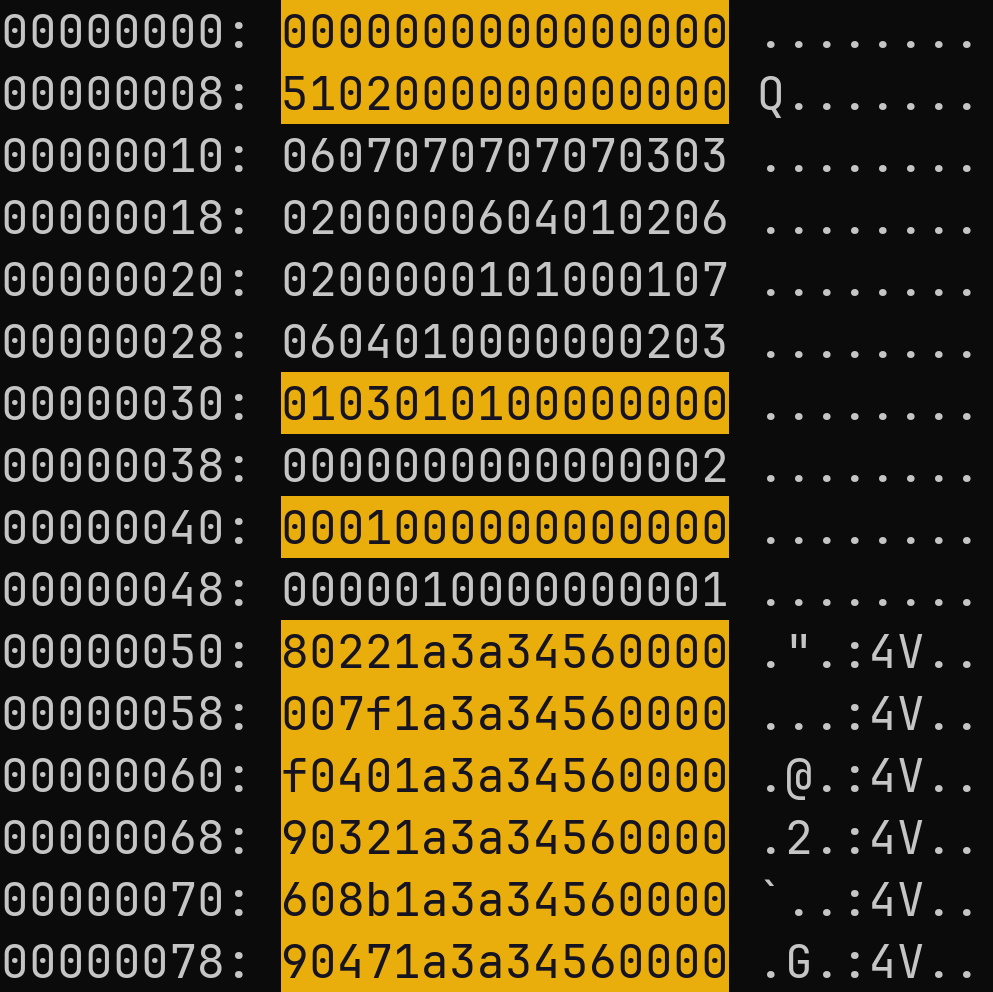
\includegraphics[width=16cm]{dataset/pointer_examples_1010-1644391327-heap_potential_pointer_highlight.png}

    We have information about the starting address of the heap using \lstinline[style=json]!"HEAP_START": "56343a198000"!. Considering that the example heap dump file contains $ 135169 $ bytes, this means that for this given heap dump file, the pointer addresses range from value $ 94782313037824_{10} $ and $ 94782313172993_{10} $. Note that the little-endian hexadecimal representation of the heap end address is \lstinline[language=c]!0x01901b3a3456! which is 12 character long, or 6 bytes long.

    Note that conversions here can get confusing, since potential pointer strings extracted from the heap dump file are given in little-endian hexadecimal format, but the heap start address from the JSON annotation file is given in big-endian hexadecimal format.

    \begin{minipage}{\dimexpr\linewidth-20pt}
        That way, we can refine the detection of potential pointers by only considering the bytes that are in the range of the heap. Potential pointers are highlighted with "<<<" in the following hex dump:

        \begin{lstlisting}[language=python, caption={Conversions function from hex strings to decimal $ int $ values}.]
        # conversion from hex to decimal
        def hex_str_to_int(hex_str: str) -> int:
            """
            Convert a normal (big-endian) hex string to an int.
            WARNING: HEAP_START in JSON is big-endian.
            """
            bytes_from_str = bytes.fromhex(hex_str)
            return int.from_bytes(
                bytes_from_str, byteorder='big', signed=False
            )
        
        def pointer_str_to_int(hex_str: str) -> int:
            """
            Convert a pointer hex string to an int.
            WARNING: Pointer hex strings are little-endian.
            """
            bytes_from_str = bytes.fromhex(hex_str)
            return int.from_bytes(
                bytes_from_str, byteorder='little', signed=False
            )
        \end{lstlisting}
    \end{minipage}

    Using the functions above, we can check which potential pointers are indeed within the heap dump range.

    \begin{minipage}{\dimexpr\linewidth-20pt}
        That way, we can refine the detection of potential pointers. In the following, pointers are highlighted with \lstinline[style=hexdump]!<<<! in the following hex dump:

        \begin{lstlisting}[style=hexdump, caption={8 bytes per line visualization of a Hex Dump from \textit{Training/basic/V\_7\_8\_P1/16/5070-1643978841-heap.raw}}]
            00000000: 0000000000000000 ........
            00000008: 5102000000000000 Q.......
            00000010: 0607070707070303 ........
            00000018: 0200000604010206 ........
            00000020: 0200000101000107 ........
            00000028: 0604010000000203 ........
            00000030: 0103010100000000 ........
            00000038: 0000000000000002 ........
            00000040: 0001000000000000 ........
            00000048: 0000010000000001 ........
            00000050: 80221a3a34560000 .".:4V.. <<<
            00000058: 007f1a3a34560000 ...:4V.. 
            00000060: f0401a3a34560000 .@.:4V.. <<<
            00000068: 90321a3a34560000 .2.:4V.. <<<
            00000070: 608b1a3a34560000 `..:4V.. <<<
            00000078: 90471a3a34560000 .G.:4V.. <<<
        \end{lstlisting}
    \end{minipage}

    \begin{minipage}{\dimexpr\linewidth-20pt}
        One last check we can do, is verify if the potential pointers are  8-bytes aligned. This can be done by checking if the last 3 bits of the potential address are 0, or using a modulo 8 operation. A simple python function can be used to check that:

        \begin{lstlisting}[language=python, caption={Python function to check if a potential pointer is 8-bytes aligned}]
            def is_pointer_aligned(pointer: int) -> bool:
                """
                Check if a pointer is 8-bytes aligned.
                """
                return pointer % 8 == 0
        \end{lstlisting}
    \end{minipage}

    Using this function on the potential pointers we have found so far, we can see that all of them are indeed 8-bytes aligned. This is a good sign for pointer detection, as we now have a range of tests that can be used to detect potential pointers from other potentially random values.

    Here is the pseudo-code for the pointer detection algorithm. This algorithm is presented for a full heap dump file:

    \begin{algorithm}
        \caption{Pointer Detection Algorithm}
        \begin{algorithmic}[1]
        \Procedure{PointerDetection}{$\text{heapDumpFile, HEAP\_START}$}
            \State $\text{heapStart} \gets \text{hex\_str\_to\_int}(HEAP\_START)$
            \State $\text{heapEnd} \gets \text{heapStart} + \text{FileSize}(\text{heapDumpFile})$
            \State $\text{position} \gets 0$
            \State $\text{potentialPointers} \gets []$
            \While{$\text{position} < \text{FileSize}(\text{heapDumpFile})$}
                \State $\text{block} \gets \text{Read8Bytes}(\text{heapDumpFile, position})$
                \If{$\text{block} \neq 0$}
                    \State $\text{pointer} \gets \text{pointer\_str\_to\_int}(\text{block})$
                    \If{$\text{heapStart} \leq \text{pointer} \leq \text{heapEnd}$}
                        \If{$\text{is\_pointer\_aligned}(\text{pointer})$}
                            \State $\text{Append}(\text{pointer}, \text{potentialPointers})$
                        \EndIf
                    \EndIf
                \EndIf
                \State $\text{position} \gets \text{position} + 8$
            \EndWhile
            \State \Return $\text{potentialPointers}$
        \EndProcedure
        \end{algorithmic}
    \end{algorithm}

    This pseudo-code outlines the steps for detecting potential pointers in the heap dump file. It starts by reading the heap dump file 8 bytes at a time. For each 8-byte block, it checks if the block is non-zero and within the heap range. If so, it checks if the potential pointer is 8-bytes aligned using the \texttt{is\_pointer\_aligned} function we described before. If all conditions are met, the potential pointer is added to the list of potential pointers. The algorithm returns this list at the end.
    
    \subsubsection{Detecting potential keys}
    % speak about SmartKex22 brute force approach
    % describe the algorithm to detect potential keys

    Encryption key prediction is the main focus of the present thesis. As such, we will now focus on how to detect potential keys in heap dump files. The paper \citetitle{SmartKex22} introduces 2 algorithms for key detection. The first one is a brute force approach that consists in trying all the possible keys in the heap dump file. The second one is a more sophisticated approach that uses a set of rules to detect potential keys.
    
    The first brute-force algorithm is given by:

    \begin{algorithm}[H]
    \caption{SSH keys brute-force algorithm from \citetitle{SmartKex22} \cite{SmartKex22}}
    \begin{algorithmic}[1]
    \Procedure{FindIVAndKey}{$\text{netPacket}, \text{heapDump}$}
        \State $\text{ivLen} \gets 16$ \Comment{Based on the encryption method}
        \State $\text{keyLen} \gets 24$ \Comment{Based on the encryption method}
        \State $i \gets \text{sizeof(cleanHeapDump)}$
        \State $r \gets 0$
        \While{$r < i$}
            \State $\text{pIV} \gets \text{heapDump}[r : r + \text{ivLen}]$
            \State $x \gets 0$
            \While{$x < i$}
                \State $\text{pKey} \gets \text{heapDump}[x : x + \text{keyLen}]$
                \State $f \gets \text{decrypt}(\text{netPacket}, \text{pIV}, \text{pKey})$
                \If{$f$ is TRUE}
                    \State \textbf{return} $\text{pIV}, \text{pKey}$
                \EndIf
                \State $x \gets x + 8$ \Comment{The IV is 8-bytes aligned}
            \EndWhile
            \State $r \gets x + 8$ \Comment{The key is 8-bytes aligned}
        \EndWhile
    \EndProcedure
    \end{algorithmic}
    \end{algorithm}
    
    Algorithm~1 outlines the brute-force approach for finding the Initialization Vector (IV) and the key. Initially, the lengths \(\text{ivLen}\) and \(\text{keyLen}\) are set based on the encryption method used for the heap. The algorithm then takes the first \(\text{ivLen}\) bytes from the heap dump to serve as the potential IV (\(pIV\)). Subsequently, \(\text{keyLen}\) bytes are extracted from the heap dump, starting from the first byte, to act as the potential key (\(pKey\)). The algorithm iterates through this potential key until it reaches the end of the heap dump. If decryption of the network packet is unsuccessful, the process is repeated by reading the next potential IV and the subsequent potential key \cite{SmartKex22}. 

    This algorithm is fairly straightforward, and can be implemented in a few lines of code. However, it is also very inefficient, as it tries all the possible keys in the heap dump file. It also needs some encrypted network packets to be able to test the keys, which are not included in the dataset. As such, we will not implement this algorithm.
    
    This is why the authors of the paper have also developed a more sophisticated algorithm that uses a set of rules to detect potential keys.

    No pseudo-code is given for the second algorithm, but the paper \citetitle{SmartKex22} gives a description of the algorithm. It rely on the high-entropy assumption of encryption keys. The algorithm is inspired by image processing techniques, and can be described as follows:

    \begin{algorithm}
        \caption{Image-processing inspired Preprocessing Algorithm, as described in \citetitle{SmartKex22} \cite{SmartKex22}}
        \begin{algorithmic}[1]
        \Procedure{Preprocessing}{$\text{heapData}$}
            \State \textbf{Reshape} $\text{heapData}$ into $N \times 8$ matrix $X$
            \For{$i = 0$ to $N-1$}
                \For{$j = 0$ to $7$}
                    \State $Y[i][j] = |X[i][j] - X[i][j+1]| \& |X[i][j] - X[i+1][j]|$
                    \State $Z[i] = \text{count}(Y[i][k] == 0) \geq 4$
                    \If{$i < N-1$}
                        \State $R[i] = Z[i] \& Z[i+1]$
                    \EndIf
                \EndFor
            \EndFor
            \State \textbf{Extract} 128-byte slices from $R$ for training
        \EndProcedure
        \end{algorithmic}
    \end{algorithm}
    
    This Preprocessing Algorithm serves as a crucial step in adapting the heap data for machine learning models. The algorithm begins by reshaping the raw heap data into an \(N \times 8\) matrix \(X\), since keys are 8-bytes aligned \cite{SmartKex22}. Here, \(N \times 8\) is the size of the original heap data in bytes. It then calculates the discrete differences of the bytes in both vertical and horizontal directions, storing the results in matrix \(Y\). The algorithm employs a logical AND operation on these differences to identify high-entropy regions, which are likely candidates for encryption keys. Each 8-byte row in \(Y\) is examined for randomness, and if at least half of its bytes differ from adjacent bytes, it is marked as a potential part of an encryption key. The algorithm then filters out isolated rows that are unlikely to be part of an encryption key, resulting in an array \(R\). Finally, 128-byte slices are extracted from \(R\) for training the machine learning model. This preprocessing step not only adapts the data for machine learning but also narrows down the search space for potential encryption keys, thereby enhancing the efficiency of the subsequent steps. 

    However, this algorithm is not as efficient as it could be. It rely on using a kind of sliding window, which is not easily parallelizable. Also, the entropy-inspired computation is not as straightforward as it could be. That why we propose a new algorithm that is more efficient and more easily parallelizable.

    In order to perform some \acrshort{ml} techniques, and because the keys we are looking for can have a range of possible lengths (16, 24, 32, or 64 bytes), we shift the focus from detecting the full key, to just be able to predict the address of the key. That way, we can deal with keys of different sizes, and we can also use the same algorithm to detect the IV. This is why we will focus on detecting potential keys addresses, and not the full keys.

    We thus introduce a new algoritm for narrowing the search space for potential keys. This algorithm is inspired by the paper \citetitle{SmartKex22}, but is more efficient and more easily parallelizable, as it focuses on producing pairs of blocks of 8 bytes with high entropy. It uses directly the Shannon entropy formula, with each entropy computation being independent from the others.

    \begin{algorithm}
        \caption{Entropy Based Detection of Potential Key blocks}
        \begin{algorithmic}[1]
        \Procedure{EntropyDetection}{$\text{heapData}$}
            \State \textbf{Pad} $\text{heapData}$ with 0s to be 8-bytes aligned
            \State \textbf{Reshape} $\text{heapData}$ into $N \times 8$ matrix $X$
            \For{$i = 0$ to $N-1$,}
                \State $entropy[i] = \text{ShannonEntropy}(X[i])$ \Comment{Independents, compute in parallel.}
            \EndFor
            \State \textbf{Add} $entropy$ 2 by 2 pairs into $entropy\_pairs$ \Comment{Keep block indexes in resulting tuples.}
            \State \textbf{Sort} $entropy\_pairs$ by entropy as $sorted\_pairs$
            \State \Return $\text{SortedPairs}(\text{sorted\_pairs})$
        \EndProcedure
        \end{algorithmic}
    \end{algorithm}

    The \textit{Entropy Based Detection of Potential Key blocks} algorithm takes a raw heap dump, represented by the variable \texttt{heapData}, as input. The data is first padded with zeros to align it to 8-byte blocks and then reshaped into an $N \times 8$ matrix $X$. The Shannon entropy is computed for each 8-byte block in parallel, resulting in an array \texttt{entropy}. Subsequently, the entropy values of adjacent blocks are summed to form pairs, which are stored in \texttt{entropy\_pairs} along with their block indexes. These pairs are then sorted by their entropy sums to produce \texttt{sorted\_pairs}. The idea of using pairs of blocks instead of a single block or more that two blocks is related to the minimim key size, which is 16 bytes. This means that we need at least 2 blocks to be able to detect a potential key. The algorithm returns sorted pairs, so that we can easily extract the ones with the highest entropy sums. Given the index of a block, its actual memory address can be recomputed using the \texttt{HEAP\_START} address available in annotations.
    
    Using this algorithm, let's continue to explore our example heap dump file from \autoref{lst:hexdump-8bytes}. We will use the following python function to compute the Shannon entropy of a given block of 8 bytes:

    \begin{minipage}{\dimexpr\linewidth-20pt}
    \begin{lstlisting}[language=python, caption={Python function to compute the Shannon entropy of a given block of 8 bytes}]
        def get_entropy(data: bytes):
            """
            Computes the entropy of a byte array, using Shannon's formula.
            """

            if len(data) == 0:
                return 0.0
            
            # Count the occurrences of each byte value
            _, counts = np.unique(data, return_counts=True)
            
            # Calculate the probabilities
            prob = counts / len(data)
            
            # Calculate the entropy using Shannon's formula
            entropy = -np.sum(prob * np.log2(prob))
            
            return entropy
    \end{lstlisting}
    \end{minipage}

    This function used np array function for efficient computation. We can now use this function to compute the entropy of each block of 8 bytes in the heap dump file. We can then sort the pair of blocks by their entropy, and keep the ones with the highest entropy.
    
    When applied to the file \textit{Training/basic/V\_7\_8\_P1/16/5070-1643978841-heap.raw}, the algorithm produced $ 16896 $ entropy pairs, with $ 631 $ pairs having the maximum entropy sum. Another test using the index to address conversion and the JSON annotation file also indicate that all of the 6 key addresses are within the $ 631 $ pairs with the highest entropy sum.
    
    This allows to reduce significantly the search space for potential keys, to already less that 4\% of the original heap dump file, which is significantly better that the 30\% reduction obtained by the preprocessing algorithm described in the paper SmartKex \cite{SmartKex22}, but less that the 2\% reduction obtained by the \acrshort{ml}-based processing algorithm described in the paper \cite{SmartKex22}. However the same paper indicated that it was tested only for Key A and Key C, whereas this algorithm is tested for all the keys. Keep in mind that this is just an example for a single random file in the dataset, as a way to introduce the subject. In-depth experiments will be done in the dedicated chapter on \acrlong{ml}.

    Indeed, it is important to mention that we can rely on the JSON annotation files for providing labelling for key address prediction. Using this, we do not need to decrypt the network packets to be able to train our \acrshort{ml} models. This is a huge advantage, and is also required since we don't have the encrypted network packets in the dataset. Since we don't have those, and since the keys are already given, that is why we will focus on key address prediction, and not on key prediction.

    \subsubsection{Detecting potential data structures}
    Since the dataset contain whole heap dump file, we can also try to detect potential data structures in those heap dumps. This can be done by looking for patterns in the heap dump file, in a similar fashion as we have done for potential pointers.
    
    Since OpenSSH is written in C, we can expect to find some C data structures in the heap dump files. C uses the \lstinline[language=c]|malloc| function to allocate memory. This function is used to allocate memory for a given data structure. This function takes as input the size of the data structure to allocate, and returns a pointer to the allocated memory. Looking at the code \footnote{The dataset has been produced on a \texttt{x86\_64} architecture, so as an example code, we have looked at uClibc for a \lstinline[language=c]|malloc| implementation: \url{https://git.busybox.net/uClibc/tree/libc/stdlib/malloc/malloc.c} } for \lstinline[language=c]|malloc|, we can see the following:
    
    \begin{minipage}{\dimexpr\linewidth-20pt}
        \begin{lstlisting}[language=c, caption={Malloc implementation for uclibc}]
        /* Include extra space to record the size of the allocated block.  */
        size += MALLOC_HEADER_SIZE;
        \end{lstlisting}
    \end{minipage}
    
    A \lstinline[language=c]|malloc| call is expected to allocate a memory block of the size of the data structure, plus 8 bytes (). This is because the \lstinline[language=c]|malloc| function also stores some metadata about the allocated memory block. This metadata is stored in the bytes that are allocated in addition to the data structure size. This is why we can expect to find some 8-bytes aligned blocks in the heap dump file, that are not pointers, but that are the result of a \lstinline[language=c]|malloc| call. Detecting and using those \textit{malloc headers} is how we will also try to detect potential data structures in the heap dump file.

    We don't know which implementation of \lstinline[language=c]|malloc| has been used for the OpenSSH programs used to generate the dataset. However, we can expect it to be similar to the one used in uclibc, a lightweight C library that is often used in embedded systems. 

    In Linux on a \texttt{x86\_64} architecture, the malloc function typically uses a block (chunk) header to store metadata about each allocated block. This header is placed immediately before the block of memory returned to the user. The exact layout can vary depending on the implementation of the C library (e.g., glibc, musl), but generally, it contains the following:

    \begin{itemize}
        \item \textbf{Size of the Block}: The size of the allocated block, usually in bytes. This size often includes the size of the header itself and may be aligned to a multiple of 8 or 16 bytes.
        \item \textbf{Flags}: Various flags that indicate the status of the block, such as whether it is free or allocated, or whether the previous block is free or allocated. These flags are often stored in the least significant bits of the size field, taking advantage of the fact that the size is usually aligned, leaving the least significant bits zeroed.
    \end{itemize}
    
    Since the malloc header respects the endianness of the system, we can expect to find the malloc header in little-endian format in the heap dump file. Using vim on \textit{Training/basic/V\_7\_8\_P1/16/5070-1643978841-heap.raw}, we can use the following command to find some potential malloc headers:

    \begin{lstlisting}[language=bash, caption={Vim command to find potential malloc headers}]
        :/[0-9a-f]\{4}0\{12}
    \end{lstlisting}
    
    This gives something like the following:

    \begin{figure}[H]
        \centering
        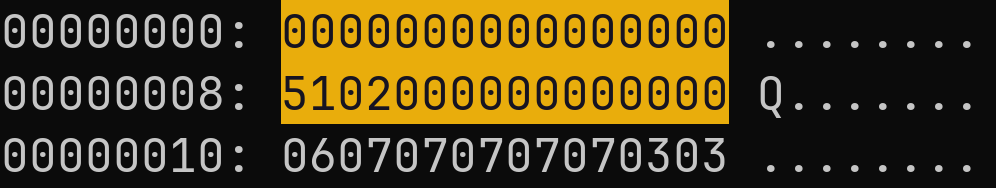
\includegraphics[width=16cm]{dataset/structure_examples_1010-1644391327-heap_potential_malloc_header_highlight_heap_start.png}
        \caption{Attempt at malloc header detection in \textit{Training/basic/V\_7\_8\_P1/16/5070-1643978841-heap.raw}, at heap start.}
    \end{figure}

    Indeed, after a first zero block of 8 bytes, we expect a first data structure to be allocated at the start of the heap. Here this data structure is of size $ 5102000000000000_{16LE} $ (little-endian hex format) or $ 593_{10} $ bytes. The fact that it is an odd number is due to the \acrshort{lsb} being set to 1, to indicate that the block is allocated (flag). This means that the real size of the structure is actually $ 593_{10} - 1_{10} = 592_{10} $. This value is 8-byte aligned.

    Since we know that the allocator allocates chunks after chunks, we can expect the next chunk to be allocated at the address $ 5102000000000000_{16LE} + 592_{10} = 5082193a34560000_{16LE} =  $. Let's have a look there:

    \begin{figure}[H]
        \centering
        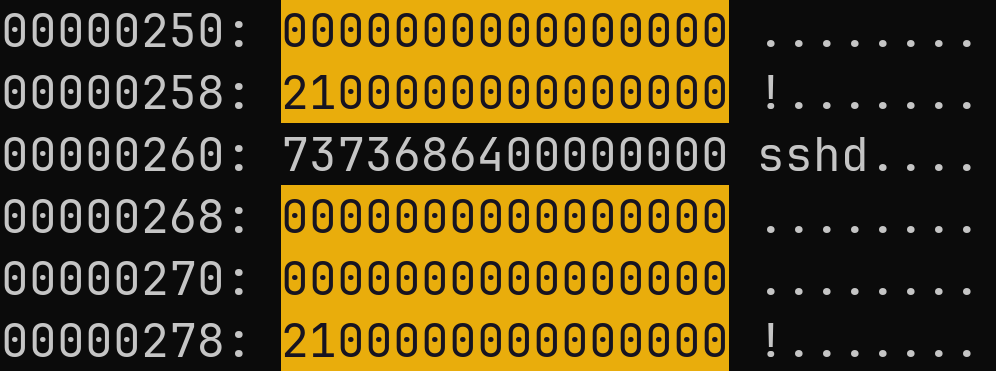
\includegraphics[width=16cm]{dataset/structure_examples_1010-1644391327-heap_potential_malloc_header_highlight_0x250.png}
        \caption{Attempt at malloc header detection in \textit{Training/basic/V\_7\_8\_P1/16/5070-1643978841-heap.raw}, at index $ 592_{10} = 250_{16} $.}
    \end{figure}

    There, we can see a zero block, followed by what we can expect to be another malloc header. By doing the same process, we can thus propose an algorithm to detect the malloc headers, and thus the structures in the heap dump file.

    \begin{algorithm}[H]
        \caption{Malloc Header Detection Algorithm}
        \begin{algorithmic}[1]
        \Procedure{MallocHeaderDetection}{$\text{heapDumpFile}$}
            \State $\text{position} \gets 0$
            \While{$\text{position} < \text{FileSize}(\text{heapDumpFile})$}
                \State $\text{block} \gets \text{Read8Bytes}(\text{heapDumpFile, position})$
                \If{$\text{block} \neq 0$}
                    \State $\text{size} \gets \text{ConvertToSize}(\text{block}) - 1$ \Comment{$-1$ due to the flag}
                    \State \textbf{Assert} $ \text{size} \mod 8 = 0$ \Comment{Check if the size is 8-bytes aligned}
                    \State $\text{position} \gets \text{position} + 8 + \text{size}$ \Comment{Leap over the data structure}
                \Else
                    \State $\text{position} \gets \text{position} + 8$
                \EndIf
            \EndWhile
        \EndProcedure
        \end{algorithmic}
    \end{algorithm}

    The idea behing the malloc header detection algorithm is simple. We start at the beginning of the heap dump file, and we look for the first non-zero block. We then assume that the next block is a malloc header. We convert it to a size, and then leap over the data structure. The process is repeated until reaching the end of the heap dump file.

    \section{Hardware and software architecture}

    \subsection{Hardware architectures}

    \subsection{Software architectures and tools}


\section{Programs development}
% describe the programs developped for the Masterarbeit
% * mem2graph

In Computer Sciences, it does't take long to realize that testing hypotheses, diving deeper in problems and finding solutions to them is a very iterative process that requires a lot of experimentation. As such, the development of scripts and programs has been a substantial part of this thesis, from the very beginning to the very end. In this process, we have used a variety of tools and programming languages, such as Rust, Python, Bash, or Nix just to name the programming language used. In this section, we will do a general overview of the programs we have developed for this thesis. More details about the programs will be discussed further in their respective chapters.


In this section, we will describe the programs we have developed for this thesis. We will first describe the program we have developed to explore the dataset. Then, we will describe the program we have developed to extract the data from the dataset. Finally, we will describe the program we have developed to analyze the data.


\section{Packaging and deployment with Nix}


Dataset in Methods Chapter: On the other hand, if the specific features and challenges of your dataset are more related to your methodology—for example, how you cleaned, balanced, or sampled the data—then these details would fit well into the Methods chapter. This is especially relevant if the issues tackled are more about "how-to" rather than "why."

